\documentclass{article}
\usepackage{tikz}
\usetikzlibrary{arrows.meta,positioning,calc,shapes.geometric}
\pagestyle{empty}
\begin{document}
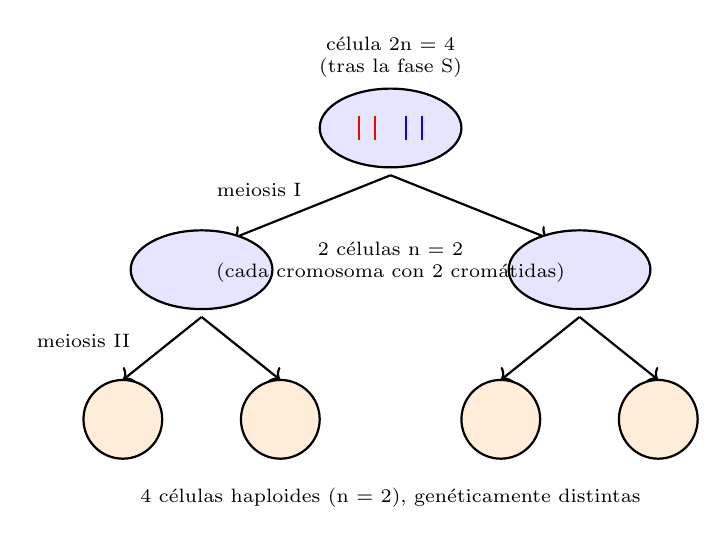
\begin{tikzpicture}
\tikzset{every node/.append style={align=center}}

\def\cellm#1#2#3{\draw[thick, fill=#3] (#1,#2) ellipse (0.9 and 0.5);}
\node[font=\scriptsize, align=center] at (0,3.6) {célula 2n = 4\\ (tras la fase S)}; \cellm{0}{2.7}{blue!10}
\draw[thick, red] (-0.4,2.55) -- (-0.4,2.85); \draw[thick, red] (-0.2,2.55) -- (-0.2,2.85); \draw[thick, blue] (0.2,2.55) -- (0.2,2.85); \draw[thick, blue] (0.4,2.55) -- (0.4,2.85);
\draw[->, thick] (0,2.1) -- (-2.0,1.3) node[midway, above left, font=\scriptsize] {meiosis I}; \draw[->, thick] (0,2.1) -- (2.0,1.3);
\cellm{-2.4}{0.9}{blue!10}\cellm{2.4}{0.9}{blue!10}
\node[font=\scriptsize, align=center] at (0,1.0) {2 células n = 2\\ (cada cromosoma con 2 cromátidas)};
\draw[->, thick] (-2.4,0.3) -- (-3.4,-0.5); \draw[->, thick] (-2.4,0.3) -- (-1.4,-0.5); \draw[->, thick] (2.4,0.3) -- (1.4,-0.5); \draw[->, thick] (2.4,0.3) -- (3.4,-0.5);
\node[font=\scriptsize] at (-3.9,0.0) {meiosis II};
\foreach \x in {-3.4,-1.4,1.4,3.4} {\draw[thick, fill=orange!15] (\x,-1.0) circle (0.5);}
\node[font=\scriptsize, align=center] at (0,-2.0) {4 células haploides (n = 2), genéticamente distintas};

\end{tikzpicture}
\end{document}
